\documentclass{article}

\usepackage[preprint]{../../neurips_2024}
\usepackage[utf8]{inputenc}
\usepackage[T1]{fontenc}
\usepackage{hyperref}
\usepackage{url}
\usepackage{booktabs}
\usepackage{graphicx}
\usepackage{amsmath}
\usepackage{amsfonts}
\usepackage{xcolor}
\usepackage{enumitem}
\usepackage{multirow}
\usepackage{tabularx}
\usepackage{array}
\usepackage{placeins}
\usepackage{tikz}
\usetikzlibrary{arrows.meta,positioning,shapes.geometric,fit}
\hypersetup{hidelinks}

\graphicspath{{../../docs/presentation/figures/}}

\makeatletter
\renewcommand{\@notice}{}
\makeatother

\newcommand{\method}[1]{\texttt{\detokenize{#1}}}
\newcommand{\dataset}[1]{\textsc{#1}}
\newcommand{\pp}{\mathrm{pp}}
\newcolumntype{Y}{>{\raggedright\arraybackslash}X}

\title{Snap-Conditioned Retrieval for Legal RAG: A Four-Benchmark Bottleneck Study}

\author{%
  Hamza Iqbal \\
  Washington University in St.\ Louis \\
  \texttt{hiqbal@wustl.edu}
  \And
  Hanson Li \\
  Washington University in St.\ Louis \\
  \texttt{hanson.l@wustl.edu}
  \And
  Josh Li \\
  Washington University in St.\ Louis \\
  \texttt{josh.l@wustl.edu}
}

\begin{document}

\maketitle

\begin{abstract}
Legal retrieval-augmented generation is often reported as a single accuracy
number: retrieve documents, generate an answer, and compare against a no-RAG
baseline. Our experiments show that this is the wrong abstraction for legal
QA. We study snap-conditioned HyDE methods across four legal benchmarks:
BarExamQA, HousingQA, LegalBench-SCALR, and CaseHOLD. Snap-conditioned HyDE
first produces a tentative legal analysis, uses it to generate a hypothetical
retrieval passage, and then answers with retrieved evidence. On full-corpus
BarExamQA, \method{rag_snap_hyde} improves Gemma 4 26B from 78.08\% to
81.17\% (+3.09pp, McNemar $p=0.0130$) and Gemma 4 E4B from 58.49\% to
62.18\% (+3.68pp, $p=0.0129$). However, the broader legal results are mixed:
BarExamQA is retrieval-depth flat, LegalBench-SCALR is candidate-depth
sensitive then saturates at top-5, HousingQA has a directional top-10
statutory-retrieval signal, and CaseHOLD improves gold-option retrieval
without a reliable answer lift. We therefore frame snap-HyDE as a useful
method family and probe, not as a universal legal RAG solution. The main
contribution of this project is a bottleneck-typed legal RAG analysis:
retrieval depth, candidate-set size, answer anchoring, metadata filtering,
and evidence-to-answer conversion must be separated before tuning methods.
\end{abstract}

\section{Introduction}

Legal QA is a natural target for retrieval augmentation. Many questions
depend on statutes, holdings, jurisdiction, procedural posture, and precise
rule exceptions that may not be reliably stored in a model's parameters.
However, legal RAG is also a setting where more retrieved text can easily
hurt. A passage can be topically related but legally incomplete; a holding can
mention the same doctrine while being the wrong option; a state statute can be
right in subject matter but wrong in jurisdiction. These errors are not just
retrieval failures or generation failures. They are interactions between
retrieval, reasoning, and answer selection.

Our initial project pursued an agentic legal RAG system: route the question to
a corpus, decompose the issue, retrieve and summarize evidence per gap, judge
sufficiency, and replan when needed. That design is realistic for legal
research, but it is difficult to evaluate scientifically. If a full agent
improves, the gain could come from better retrieval, more tokens, a second
reasoning pass, or a lucky prompt. If it fails, the error could come from
over-decomposition, bad gap detection, irrelevant evidence, or answer
overwriting. We therefore moved from full-system complexity to atomic
retrieval interventions.

The central method family is snap-conditioned HyDE. A ``snap'' is a first-pass
answer or reasoning trace. A HyDE-style hypothetical passage is then generated
from that snap and used for retrieval. The final answer sees the question,
snap reasoning, and retrieved evidence. The intuition is legal: before asking
the model to read external authority, ask it to state the issue and likely
rule. Retrieval is then shaped by that legal frame rather than by the raw
question alone.

The current legal-only evidence is not uniformly positive, and that is useful.
BarExamQA shows a real full-corpus snap-HyDE lift, but top-1 versus top-5
retrieval is flat, so the lift should not be described as ``more documents
help.'' LegalBench-SCALR shows a strong top-1 collapse and top-5 saturation,
which suggests candidate-set size matters more than pseudo-document query
formulation. HousingQA has a promising top-10 signal, but a state-filter run
failed due a metadata-casing bug and remains pending after repair. CaseHOLD
now has repaired gold-option retrieval, and snap-HyDE raises gold retrieval
from 16.0\% to 47.0\%, but answer accuracy only moves from 69.5\% to 72.0\%
with $p=0.4421$.

We exclude MuSiQue from the main report because it is not a legal benchmark.
It remains a useful internal multi-hop mechanism check, but the final class
report is framed around four legal benchmarks. This makes the narrative less
numerically convenient, because the strongest two-call snap-HyDE lift in the
repo is currently on MuSiQue. That is acceptable for the current stage. The
goal is to identify which legal bottlenecks are real, then tune retrieval and
HyDE quality toward those bottlenecks.

\section{Related Work}

Retrieval-augmented generation combines parametric generation with retrieved
non-parametric evidence \citep{lewis2020rag}. HyDE generates a hypothetical
document and embeds it for zero-shot retrieval \citep{gao2023hyde}, while
Query2Doc expands queries with LLM-generated pseudo-documents
\citep{wang2023query2doc}. FLARE retrieves during generation by using
predicted future content as a query \citep{jiang2023flare}. Our method family
inherits directly from this line: generated text is used as a retrieval
handle, not as trusted evidence.

Adaptive RAG work asks when or how retrieval should be invoked. Self-RAG
learns to retrieve and critique through reflection tokens
\citep{asai2024selfrag}. Corrective RAG grades retrieved evidence and triggers
correction when retrieval is unreliable \citep{yan2024crag}. Adaptive-RAG
routes questions by complexity \citep{jeong2024adaptive}. Speculative RAG
drafts multiple answers from retrieved subsets and verifies them with a larger
model \citep{wang2025specrag}. These systems motivate our future direction,
but we do not claim to implement them here. Instead, we use their shared
lesson: retrieval should be conditional on observed failure mode.

Legal NLP benchmarks increasingly show that legal RAG cannot be reduced to
generic open-domain QA. LegalBench provides a broad suite of legal reasoning
tasks, including SCALR holding selection \citep{guha2023legalbench}.
CaseHOLD evaluates whether a model can select the holding referenced by a
court-opinion context \citep{zheng2021casehold}. Zheng et al.\ introduce
BarExamQA and Housing Statute QA to evaluate realistic legal retrieval and
answering workflows \citep{zheng2025legalretrieval}. LegalBench-RAG focuses on
retrieving minimal relevant legal snippets \citep{pipitone2024legalbenchrag},
and Legal RAG Bench provides an end-to-end legal RAG benchmark with factorial
retriever/generator decomposition \citep{butler2026legalragbench}. RAGChecker
similarly argues for fine-grained separation of retrieval and generation
errors \citep{ru2024ragchecker}. Our work follows this diagnostic turn: the
same RAG method should be judged differently depending on whether the active
failure is retrieval depth, candidate-set selection, metadata filtering, or
evidence conversion.

We also considered hypothetical-representation work beyond HyDE. HyQE ranks
contexts with hypothetical query embeddings \citep{zhou2024hyqe}. We did not
implement a separate ``HyRE'' or hypothetical reasoning embedding index in
this report. The implemented object is simpler: online snap-conditioned HyDE
used as a legal retrieval probe.

\section{Framework Design}

\subsection{Method ladder}

The report uses an inheritance-style method ladder. Each method adds one
capability where possible, so negative rows remain interpretable.

\begin{center}
\small
\begin{tabularx}{\textwidth}{lY}
\toprule
Method & What it isolates \\
\midrule
\method{llm_only} & Parametric legal answer without retrieval. \\
\method{snap_only_in_final} & Whether a first-pass answer/reasoning trace helps without retrieval. \\
\method{rag_simple} & Standard retrieval plus answer generation. \\
\method{rag_hyde} & Question-conditioned hypothetical document retrieval. \\
\method{rag_snap_hyde} & Snap-conditioned HyDE retrieval plus final synthesis. \\
\method{rag_snap_hyde_1call} & Whether snap reasoning alone after ordinary retrieval is enough. \\
\method{rag_snap_hyde_2call} & Fixed-cost snap and HyDE passage in one first call, final synthesis in a second. \\
\method{multi_hyde_diverse} & Multiple generated retrieval passages for query diversity. \\
\method{subagent_rag} & Gap-routed report generation; currently used as a negative over-abstention control. \\
\bottomrule
\end{tabularx}
\end{center}

\subsection{Snap-conditioned HyDE}

Figure~\ref{fig:method_diagram} shows the core method. The model first writes
a snap answer or legal analysis. It then writes a hypothetical passage that
states the likely controlling rule, fact, or holding. That passage is embedded
and used for retrieval. The final model sees retrieved passages along with
the original question and snap reasoning.

\begin{figure}[!htbp]
\centering
\resizebox{\textwidth}{!}{%
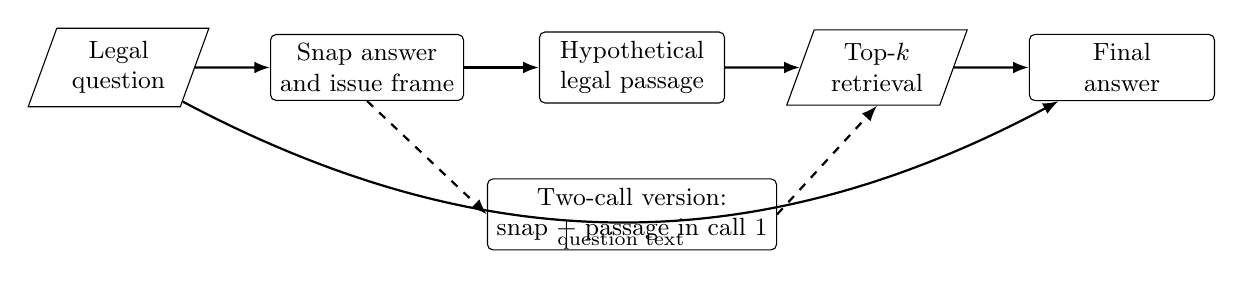
\begin{tikzpicture}[
  node distance=0.85cm and 0.95cm,
  box/.style={draw, rounded corners=2pt, minimum width=2.35cm, minimum height=0.72cm, align=center, font=\small},
  data/.style={draw, trapezium, trapezium left angle=70, trapezium right angle=110, minimum width=2.3cm, minimum height=0.72cm, align=center, font=\small},
  arr/.style={-{Latex[length=2mm]}, thick}
]
\node[data] (q) {Legal\\question};
\node[box, right=of q] (snap) {Snap answer\\and issue frame};
\node[box, right=of snap] (hyde) {Hypothetical\\legal passage};
\node[data, right=of hyde] (ret) {Top-$k$\\retrieval};
\node[box, right=of ret] (final) {Final\\answer};
\draw[arr] (q) -- (snap);
\draw[arr] (snap) -- (hyde);
\draw[arr] (hyde) -- (ret);
\draw[arr] (ret) -- (final);
\draw[arr] (q) to[bend right=28] node[below,font=\scriptsize]{question text} (final);
\node[box, below=0.95cm of hyde, minimum width=3.4cm] (twocall) {Two-call version:\\snap + passage in call 1};
\draw[arr, dashed] (snap.south) -- (twocall.west);
\draw[arr, dashed] (twocall.east) -- (ret.south);
\end{tikzpicture}}
\caption{Snap-conditioned HyDE. The generated passage shapes retrieval; the
retrieved corpus passages remain the external evidence used by final
synthesis.}
\label{fig:method_diagram}
\end{figure}

\subsection{Bottleneck diagnostics}

We use three families of diagnostics. First, top-$k$ sensitivity tests whether
answer accuracy depends on retrieving more than the single best passage. This
is a retrieval-policy stress test, not pure context truncation, because the
cross-encoder reranks a first-stage candidate pool before selecting the final
top-$k$. Second, snap-only and HyDE-only ablations ask whether the gain comes
from answer anchoring, generated-query retrieval, or their combination. Third,
gold-retrieval and disagreement audits ask whether better retrieval actually
converts into better final answers.

The four legal benchmarks map naturally onto different bottleneck hypotheses:
BarExamQA tests answer anchoring under strong legal priors, HousingQA tests
jurisdiction-specific statutory retrieval, LegalBench-SCALR tests small
candidate-set holding selection, and CaseHOLD tests whether a retrieved
holding can be converted into the correct answer option.

\section{Experimental Setup}

\paragraph{Benchmarks.}
BarExamQA contains 1,195 bar-exam multiple-choice questions with fact patterns
and legal passages. HousingQA contains yes/no housing-law questions over state
statutes. LegalBench-SCALR contains 571 Supreme Court holding-selection
questions. CaseHOLD contains court-opinion contexts and five candidate
holdings. We deliberately exclude non-legal MuSiQue from the main benchmark
set, although it remains useful for internal multi-hop stress testing.

\paragraph{Models.}
The full-corpus BarExamQA rows use Gemma 4 26B-A4B and Gemma 4 E4B served
through cluster logs. LegalBench-SCALR and CaseHOLD diagnostic rows use Llama
70B. HousingQA uses Gemma 4 26B. For paired claims, we compare runs on the
same question slice and provider. The laptop Chroma checkout is useful for
SCALR smoke tests, but it is not the availability boundary for this project:
the cluster checkout contains the larger legal collections, so BarExamQA,
HousingQA, CaseHOLD, and SCALR follow-up retrieval runs are launched through
SLURM when they need populated corpora.

\paragraph{Metrics.}
We report accuracy for multiple-choice and yes/no datasets. Paired deltas use
exact McNemar tests with b/c discordance counts. Retrieval diagnostics report
gold retrieval only when the dataset's gold mapping and corpus collection are
known to be valid. All headline rows in this draft were re-checked against
detail logs in \texttt{reports/final\_class\_report/evidence\_snapshot.md}.

\section{Results and Analysis}

\subsection{BarExamQA: full-corpus snap-HyDE lift}

BarExamQA is the strongest legal positive result. On Gemma 4 26B-A4B,
\method{rag_snap_hyde} reaches 81.17\%, compared with 78.08\% for
\method{rag_simple} (+3.09pp, b/c=124/87, $p=0.0130$). On Gemma 4 E4B, the
same method improves 58.49\% to 62.18\% (+3.68pp, b/c=172/128,
$p=0.0129$).

\begin{table}[!htbp]
\centering
\caption{BarExamQA full-corpus Gemma 4 26B-A4B method matrix, $N=1195$.}
\label{tab:barexam}
\small
\begin{tabular}{lcc}
\toprule
Method & Accuracy & $\Delta$ vs \method{rag_simple} \\
\midrule
\method{rag_simple} & 78.08\% & -- \\
\method{golden_passage} & 78.66\% & +0.58pp \\
\method{rag_hyde} & 78.91\% & +0.83pp \\
\method{llm_only} & 79.75\% & +1.67pp \\
\method{snap_only_in_final} & 80.59\% & +2.51pp \\
\textbf{\method{rag_snap_hyde}} & \textbf{81.17\%} & \textbf{+3.09pp} \\
\bottomrule
\end{tabular}
\end{table}

The mechanism is not pure retrieval depth. On a paired $N=200$ diagnostic,
\method{rag_simple} top-5 is 82.5\% and top-1 is 83.0\% ($p=1.0$). The
full-corpus lift is better read as snap answer anchoring and evidence
reconciliation. A legal MC model can have strong prior knowledge of the rule;
retrieval then helps only if it is framed in a way that does not overwrite the
right legal analysis with a partial snippet.

\begin{figure}[!htbp]
  \centering
  
\includegraphics[width=0.70\textwidth]{02_barexam_cross_size.png}
  \caption{BarExamQA cross-size result. \method{rag_snap_hyde} improves over
  \method{rag_simple} on both Gemma 4 model sizes.}
  \label{fig:barexam_cross_size}
\end{figure}

\subsection{Four-benchmark legal bottleneck matrix}

Table~\ref{tab:legal_matrix} is the compact result summary. It intentionally
includes negative and directional rows. The current evidence does not show
one method winning everywhere; it shows which legal bottleneck each dataset is
probing.

\begin{table}[!htbp]
\centering
\caption{Legal-only benchmark matrix. MuSiQue is excluded because it is not
legal-domain data.}
\label{tab:legal_matrix}
\footnotesize
\begin{tabularx}{\textwidth}{p{0.18\textwidth}p{0.25\textwidth}p{0.27\textwidth}Y}
\toprule
Benchmark & Snap-HyDE / method result & Depth or retrieval diagnostic & Current read \\
\midrule
BarExamQA / Gemma 4 &
Full $N=1195$: +3.09pp at 26B, +3.68pp at E4B &
top-5 82.5\% vs top-1 83.0\%, flat &
Legal MC is answer-anchoring dominated, not depth limited. \\
\addlinespace
HousingQA / Gemma 4 &
\method{rag_snap_hyde_2call} 57.0\% at k=5 &
top-1 50.5\% to top-10 58.0\%, +7.5pp, $p=0.0722$ &
Directional statutory-depth signal; state filtering is pending. \\
\addlinespace
LegalBench-SCALR / Llama 70B &
\method{rag_snap_hyde_2call} 75.0\% vs \method{rag_simple} 77.0\%, NS &
top-1 59.5\%, top-5 77.0\%, top-10 77.0\% &
Candidate-set limited until top-5, then saturated. \\
\addlinespace
CaseHOLD / Llama 70B &
Repaired pair: 69.5\% to 72.0\%, $p=0.4421$ &
top-1 64.5\%, top-5 69.5\%; gold retrieval 9.0\%, 16.0\%, 47.0\% under two-call &
Some depth signal, but better gold retrieval does not yet convert to reliable answer lift. \\
\bottomrule
\end{tabularx}
\end{table}

The most important negative result is CaseHOLD. After repairing the holdings
corpus and gold mapping, top-1 \method{rag_simple} reaches 64.5\% with 9.0\%
gold retrieval, while top-5 reaches 69.5\% with 16.0\% gold retrieval
(+5.0pp, $p=0.0525$). Two-call snap-HyDE then raises gold retrieval to 47.0\%
but answer accuracy only reaches 72.0\% ($p=0.4421$ against top-5
\method{rag_simple}). If retrieval recall were sufficient, answer accuracy
should improve sharply. It does not. This suggests an evidence-to-option
bottleneck: retrieved holdings can still be paraphrased distractors, overly
generic, or hard to map back to the exact candidate label.

SCALR gives a different holding-selection story. Top-1 is poor, top-5 fixes
most of the loss, and top-10 adds no answer accuracy beyond top-5. This is not
a generic ``legal holdings ignore retrieval'' result. It says SCALR needs a
small candidate set, while CaseHOLD needs better evidence conversion.

HousingQA is the most important unfinished legal retrieval result. The top-10
lift is directionally positive, but the state-filter experiment failed because
question states were display-case strings while Chroma metadata was lowercase.
That is an infrastructure bug, not a method result. The fixed state-filter run
is pending; until then, HousingQA supports only a cautious statutory-depth
claim.

\subsection{Gold passage is not an oracle in legal MC}

The BarExamQA golden-passage control appears paradoxical: providing the gold
passage reaches only 78.66\%, below \method{llm_only} at 79.75\% and
\method{snap_only_in_final} at 80.59\%. The reason is legal evidence
granularity. A labeled passage can be topically correct but not decisive for
the fact pattern; it can also highlight a distractor doctrine. Snap-first
reasoning gives the model an initial legal frame before evidence
reconciliation, which partly protects against over-reading one snippet.

\begin{figure}[!htbp]
  \centering
  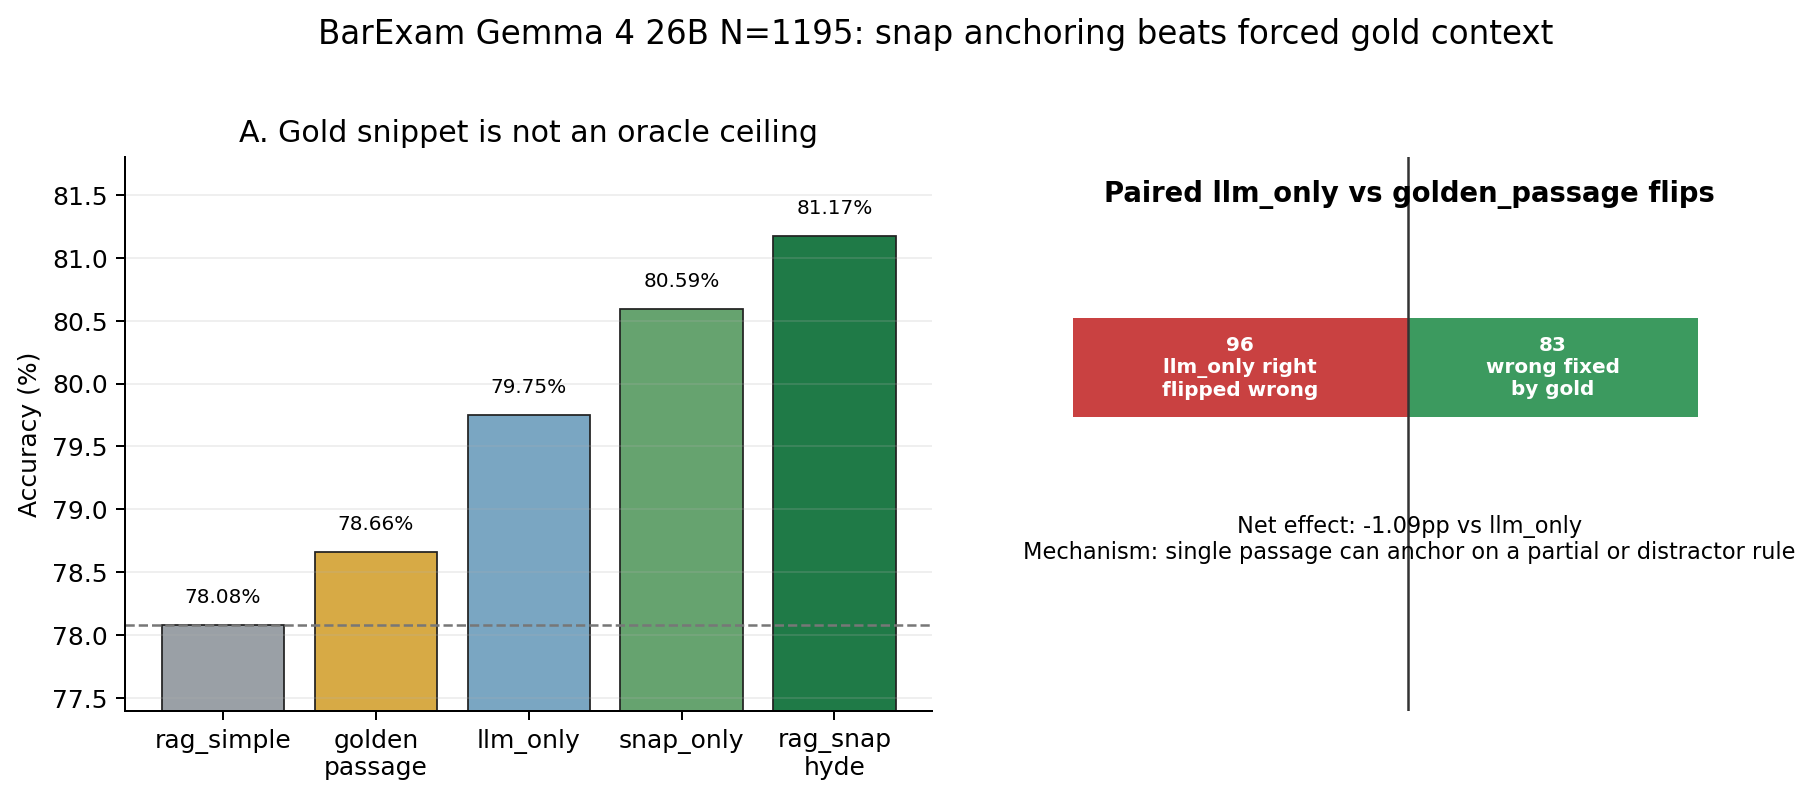
\includegraphics[width=0.82\textwidth]{11_barexam_golden_snap_mechanism.png}
  \caption{BarExamQA mechanism audit. A single gold passage is a noisy control
  rather than an oracle ceiling; snap-first reasoning can recover some cases
  where forced context distracts the model.}
  \label{fig:golden_mechanism}
\end{figure}

\subsection{Current follow-up runs}

The next legal-only runs are now cluster-backed rather than laptop-limited.
The active set is:

\begin{center}
\small
\begin{tabularx}{\textwidth}{lY}
\toprule
Job & Purpose \\
\midrule
SLURM 58799 & HousingQA state-filtered retrieval at k=5 and k=10 after fixing
the state-metadata casing bug. \\
SLURM 58871 & CaseHOLD repaired top-k follow-up: \method{rag_simple} at k=1
has landed at 64.5\%; k=10 plus \method{rag_hyde} at k=5 remain in progress. \\
SLURM 58885 & LegalBench-SCALR snap ablation: \method{rag_hyde} and
\method{rag_snap_hyde_1call} at k=5, complementing existing
\method{rag_simple} and \method{rag_snap_hyde_2call} rows. \\
\bottomrule
\end{tabularx}
\end{center}

BarExamQA already has full-corpus snap-HyDE evidence, so the immediate
priority is not another broad BarExamQA sweep. The useful BarExamQA add-on is
a narrower generated-query ablation, such as \method{multi_hyde_diverse}, if
API budget remains after HousingQA and CaseHOLD complete.

\section{Discussion: From Method Search to Bottleneck Routing}

The most useful interpretation of these results is not that snap-HyDE is the
final method. It is that a small family of fixed interventions can expose
which part of a legal RAG pipeline is currently binding. This matters because
many RAG papers collapse several different phenomena into one comparison:
retrieval versus no retrieval. In our logs, that comparison is too coarse.
LegalBench-SCALR loses heavily at top-1 and recovers at top-5, so a route that
expands the candidate set is plausible. BarExamQA is top-$k$ flat but improves
with snap-conditioned final synthesis, so the route should preserve an answer
frame rather than simply retrieve more passages. HousingQA likely requires
metadata-constrained statutory retrieval, because the question state is part
of the legal problem. CaseHOLD improves gold retrieval under two-call
snap-HyDE but not answer accuracy, so the route should focus on mapping
retrieved holdings back to answer options.

This gives a feasible version of the ``agentic'' idea without making the
agent itself the unit of evaluation. Instead of asking a planner to invent an
open-ended research workflow, we can ask a controller to choose among a small
set of evidence-budgeted interventions. The controller would observe cheap
features before or during retrieval: question type, answer format, available
metadata, top-score margin, retrieved-document agreement, candidate-option
similarity, and whether the snap answer agrees with retrieval. It would then
choose a route: ordinary RAG, top-$k$ expansion, snap-conditioned HyDE,
state-filtered retrieval, multi-query diversity, or option-aware reranking.
The result is still agentic in the sense that method adaptation happens on the
fly, but it is experimentally cleaner because every route corresponds to a
measured ablation cell.

\begin{center}
\small
\begin{tabularx}{\textwidth}{p{0.21\textwidth}p{0.28\textwidth}Y}
\toprule
Observed signal & Likely bottleneck & Route to test next \\
\midrule
Top-1 fails, top-5 recovers, top-10 flat &
Candidate-set size rather than answer reasoning &
Use top-5 as default; spend budget on reranking or option grounding instead
of deeper context. \\
\addlinespace
Snap-only beats or matches retrieval &
Evidence is distracting or under-specified relative to legal priors &
Keep a first-pass legal frame in final synthesis and audit whether evidence
overwrites correct priors. \\
\addlinespace
Generated retrieval improves gold-hit but not answer accuracy &
Evidence-to-answer conversion bottleneck &
Add answer-option-aware synthesis, contradiction checks, or verifier scoring
rather than more retrieval. \\
\addlinespace
Question contains jurisdiction metadata &
Corpus filtering and metadata normalization bottleneck &
Filter before retrieval, validate non-empty evidence, and compare against
generic top-$k$ retrieval. \\
\addlinespace
Retriever scores are low or retrieved passages disagree &
Query formulation bottleneck &
Try snap-HyDE or diverse HyDE passages, then measure whether gold retrieval
and answer accuracy move together. \\
\bottomrule
\end{tabularx}
\end{center}

This framing also explains why the current negative results are useful. A
negative CaseHOLD answer delta after a positive gold-hit delta is not just a
failed method row; it identifies a downstream conversion problem. A flat
BarExamQA top-$k$ sweep does not make retrieval irrelevant; it says that
retrieval depth is not the active lever for that slice. A pending HousingQA
state-filter result is not a missing number to hide; it is exactly the kind of
metadata gate a legal RAG system must satisfy before its answers can be
trusted. These are the hooks for a stronger final project: tune snap-HyDE
quality where query formulation is binding, tune metadata filters where
jurisdiction is binding, and tune verifier or option-mapping logic where
evidence conversion is binding.

The class-report claim is therefore deliberately modest but concrete. We built
and audited a legal RAG harness that can run comparable methods across several
legal benchmarks; we found one full-corpus legal snap-HyDE lift on BarExamQA;
we found several $N=200$ diagnostic signals that disagree with a single-method
story; and we turned those signals into a routing agenda. That is a better
foundation for future work than another broad sweep over loosely comparable
prompts, because it says what should change when a method fails.

\section{Limitations and Future Work}

The report is intentionally conservative. Only BarExamQA has a full-corpus
legal result. HousingQA, SCALR, and CaseHOLD are paired $N=200$ diagnostic
slices. These are useful for mechanism discovery and class-report evidence,
but they are not final benchmark claims. HousingQA also has an unresolved
metadata-filter gate: the first state-filter job produced empty retrieval and
must not be cited as a method result.

The current method set is incomplete relative to the literature. We define
Self-RAG, CRAG, and Speculative RAG, but do not reimplement them. We also do
not yet log true Speculative-RAG draft/verifier metrics. The local HyDE
methods need improvement: better corpus-style passage prompts, explicit
jurisdiction handling for HousingQA, and answer-option-aware final synthesis
for holding tasks. The goal is not to defend the current numbers as final; it
is to use them to identify where tuning should be applied.

The next experiments should stay legal-only. First, finish HousingQA
state-filtered retrieval and compare it to top-10 generic retrieval. Second,
add SCALR \method{rag_hyde}, \method{rag_snap_hyde_1call}, and
\method{multi_hyde_diverse} rows if API budget allows. Third, finish repaired
CaseHOLD k=10 and \method{rag_hyde} after the Chroma repair so the depth-policy
claim uses meaningful gold retrieval. Fourth, if we want a stronger retrieval
benchmark, wire LegalBench-RAG or Legal RAG Bench rather than adding another
generic multi-hop dataset.

\section{Conclusion}

The legal-only evidence supports a bottleneck-typed view of RAG. Snap-HyDE
helps BarExamQA at full corpus, but BarExamQA is not retrieval-depth limited.
SCALR is candidate-depth limited, HousingQA is a pending statutory metadata
test, and CaseHOLD shows that better retrieval does not automatically convert
to better answers. These mixed results are not a failure of the project. They
are the project signal: before building a bigger agent or declaring a RAG
method better, we need to know whether the legal task needs more candidates,
better generated queries, state-aware filtering, answer anchoring, or a
stronger evidence-to-option mapper.

\clearpage
\bibliographystyle{plainnat}
\bibliography{references}

\end{document}
